%package list
\documentclass{article}
\usepackage[top=3cm, bottom=3cm, outer=3cm, inner=3cm]{geometry}
\usepackage{multicol}
\usepackage{graphicx}
\usepackage{url}
%\usepackage{cite}
\usepackage{hyperref}
\usepackage{array}
\usepackage{bookmark}
%\usepackage{multicol}
\newcolumntype{x}[1]{>{\centering\arraybackslash\hspace{0pt}}p{#1}}
\usepackage{natbib}
\usepackage{pdfpages}
\usepackage{multirow}
\usepackage[normalem]{ulem}
\useunder{\uline}{\ul}{}
\usepackage{xcolor}

%\usepackage{booktabs}
\usepackage[labelformat=empty]{caption}
\usepackage{subcaption}
\usepackage{float}
\usepackage{array}
\usepackage{minted}

\setminted{fontsize=\small,numbers=left,autogobble}
\newenvironment{block}{\captionsetup{type=listing}}{}

\newcolumntype{M}[1]{>{\centering\arraybackslash}m{#1}}
\newcolumntype{N}{@{}m{0pt}@{}}

% para el codigo fuente
\usepackage{listings}
\usepackage{color, colortbl}
\definecolor{dkgreen}{rgb}{0,0.6,0}
\definecolor{gray}{rgb}{0.5,0.5,0.5}
\definecolor{mauve}{rgb}{0.58,0,0.82}
\definecolor{codebackground}{rgb}{0.95, 0.95, 0.92}
\definecolor{tablebackground}{rgb}{0.8, 0, 0}

\lstset{frame=tb,
	language=bash,
	aboveskip=3mm,
	belowskip=3mm,
	showstringspaces=false,
	columns=flexible,
	basicstyle={\small\ttfamily},
	numbers=none,
	numberstyle=\tiny\color{gray},
	keywordstyle=\color{blue},
	commentstyle=\color{dkgreen},
	stringstyle=\color{mauve},
	breaklines=true,
	breakatwhitespace=true,
	tabsize=3,
	backgroundcolor= \color{codebackground},
}

%Comando
\newcommand{\itemEmail}{mjarama@unsa.edu.pe}
\newcommand{\itemStudent}{Mariel Alisson Jara Mamani}
\newcommand{\itemStudentShort}{Mariel Jara}
\newcommand{\itemCourse}{Programación Web 2}
\newcommand{\itemCourseCode}{1702122}
\newcommand{\itemSemester}{I}
\newcommand{\itemUniversity}{Universidad Nacional de San Agustín de Arequipa}
\newcommand{\itemFaculty}{Facultad de Ingeniería de Producción y Servicios}
\newcommand{\itemDepartment}{Departamento Académico de Ingeniería de Sistemas e Informática}
\newcommand{\itemSchool}{Escuela Profesional de Ingeniería de Sistemas}
\newcommand{\itemAcademic}{2023 \- B}
\newcommand{\itemInput}{Del 3 Junio 2024}
\newcommand{\itemOutput}{Al 6 Junio 2024}
\newcommand{\itemPracticeNumber}{09}
\newcommand{\itemTheme}{Angular}
\renewcommand{\contentsname}{Laboratorio \itemPracticeNumber}
%%%%%%%%%%%%%%%%%%%%%%%%%%%%%%%%%%%%%%%%%%%%%%%%%%%%%%%%%%%%%%%%%%%%%%%%%%%%
%%%%%%%%%%%%%%%%%%%%%%%%%%%%%%%%%%%%%%%%%%%%%%%%%%%%%%%%%%%%%%%%%%%%%%%%%%%%

\usepackage[utf8]{inputenc}
\renewcommand{\figurename}{Figura}
\renewcommand{\refname}{Referencias}
\renewcommand{\tablename}{Tabla} %esto no funciona cuando se usa babel
\AtBeginDocument{%
\renewcommand\tablename{Tabla}
\setlength{\headheight}{40.51407pt}
}

\usepackage{fancyhdr}
\pagestyle{fancy}
\fancyhf{}
\setlength{\headheight}{30pt}
\renewcommand{\headrulewidth}{1pt}
\renewcommand{\footrulewidth}{1pt}
\fancyhead[L]{\raisebox{-0.2\height}{
\includegraphics[width=3cm]{img/episunsa.png}}}
\fancyhead[C]{\fontsize{7}{7}\selectfont	\itemUniversity \\ \itemFaculty \\ \itemDepartment \\ \itemSchool\\\textbf{\itemCourse}}
\fancyhead[R]{\raisebox{-0.2\height}{
\includegraphics[width=1.2cm]{img/logo_abet.png}}}
\fancyfoot[L]{\itemStudentShort}
\fancyfoot[C]{\itemCourse}
\fancyfoot[R]{Página \thepage}

\begin{document}

\vspace*{10px}

\begin{center}
	\fontsize{17}{17} \textbf{ Informe de Laboratorio \itemPracticeNumber}
\end{center}
\centerline{\textbf{\Large Tema: \itemTheme}}
%\vspace*{0.5cm}	

\begin{flushright}
	\begin{tabular}{|M{2.5cm}|N|}
		\hline
		\rowcolor{tablebackground}
		\color{white} \textbf{Nota} \\
		\hline
		\\[30pt]
		\hline
	\end{tabular}
\end{flushright}

\begin{table}[H]
	\begin{tabular}{|M{5.4cm}|M{4.0cm}|M{4.7cm}|}
		\hline
		\rowcolor{tablebackground}
		\color{white} \textbf{Estudiante(s)} & \color{white}\textbf{Escuela} & \color{white}\textbf{Asignatura}                                        \\
		\hline
		{\itemStudent \par \itemEmail}       & \itemSchool                   & {\itemCourse \par Semestre: \itemSemester \par Código: \itemCourseCode} \\
		\hline
	\end{tabular}
\end{table}

\begin{table}[H]
	\begin{tabular}{|M{4.7cm}|M{4.7cm}|M{4.7cm}|}
		\hline
		\rowcolor{tablebackground}
		\color{white}\textbf{Laboratorio} & \color{white}\textbf{Tema} & \color{white}\textbf{Duración} \\
		\hline
		\itemPracticeNumber               & \itemTheme                 & 04 horas                       \\
		\hline
	\end{tabular}
\end{table}

\begin{table}[H]
	\begin{tabular}{|M{4.7cm}|M{4.7cm}|M{4.7cm}|}
		\hline
		\rowcolor{tablebackground}
		\color{white}\textbf{Semestre académico} & \color{white}\textbf{Fecha de inicio} & \color{white}\textbf{Fecha de entrega} \\
		\hline
		\itemAcademic                            & \itemInput                            & \itemOutput                            \\
		\hline
	\end{tabular}
\end{table}
\pagebreak

\tableofcontents
\pagebreak


%%%%%%%%%%%%%%%%%%%%%%%%%%%%%%%%%%%%%%%%%%%%%%%%%%%%%%%%%%%%%%%%%%%%%%
\section{Tarea}
\begin{itemize}
	\item \textbf{Ejercicio 1:}
	      \begin{itemize}
		      \item Se desea crear un proyecto con Angular que implemente el juego del ahorcado.  Se tendrá un arreglo con posibles palabras a adivinar por parte del usuario.  La interfaz la dejamos a gusto de ustedes los programadores.
	      \end{itemize}
	\item \textbf{Observaciones:}
	      \begin{itemize}
		      \item Forme grupos de 2 a 4 personas
		      \item Reportar al profesor que logró culminar la tarea. La tarea debe ser compartida con el profesor en github (CarloCorrales010) y entregada usando el mismo url que se usó para clonar el repositorio. Además cada integrante del grupo deberá crear un video de 5 minutos en flipgrid explicando la aplicación.
	      \end{itemize}
\end{itemize}
\pagebreak
%%%%%%%%%%%%%%%%%%%%%%%%%%%%%%%%%%%%%%%%%%%%%%%%%%%%%%%%%%%%%%%%%%%%%%
\section{Commits}
\begin{figure}[H]
	\centering
	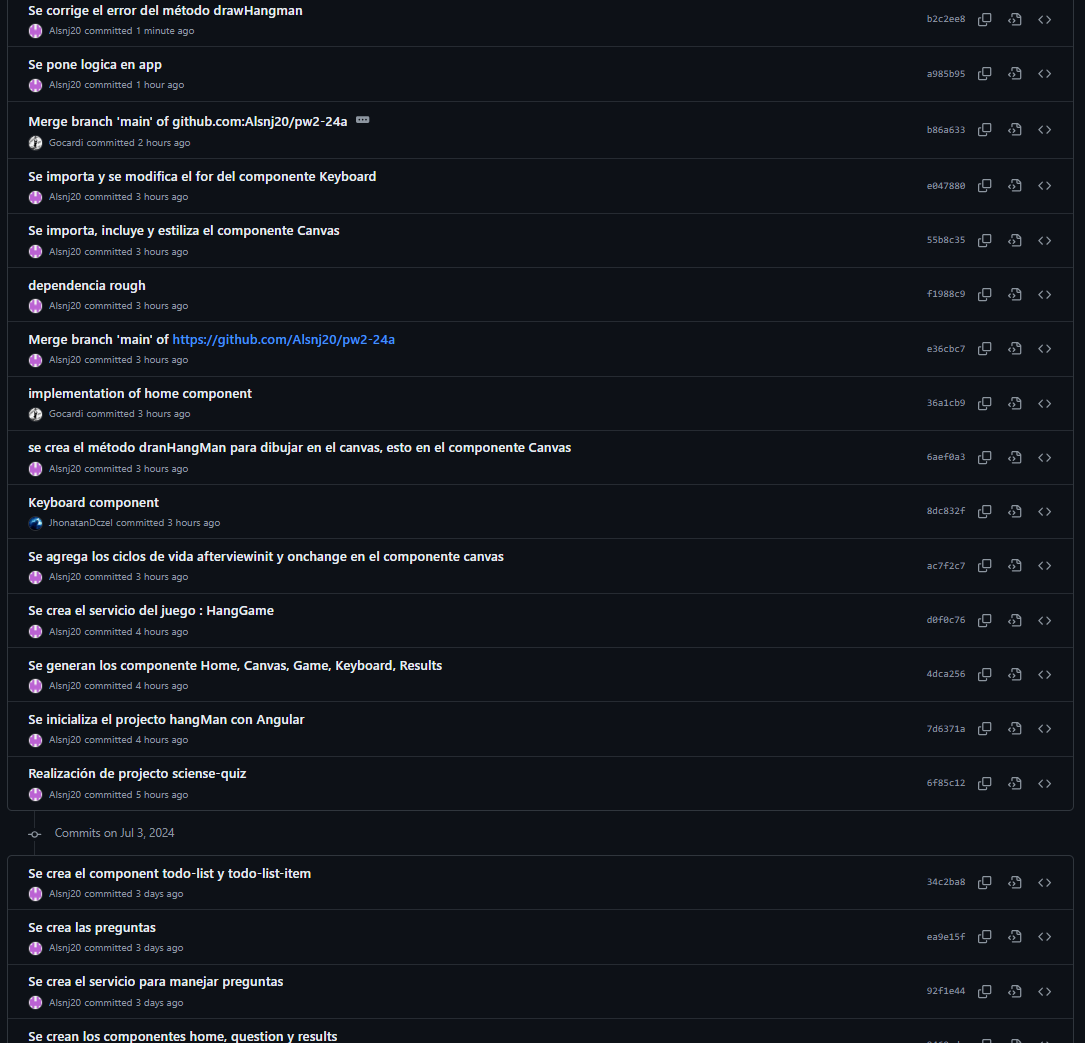
\includegraphics[width=0.9\textwidth,keepaspectratio]{img/commits.png}
	\caption{Lista de commits realizados en el proyecto.}
\end{figure}
\pagebreak
\section{Equipos y materiales utilizados}
\begin{itemize}
	%%%%%%%%%%%%%%%%%%%%%%%%%%%%%%%%%%%%%%%%%%%%%%%%%%%%%%%%%%%%%%%%%%%%%%
	\item Cuenta en GitHub con el correo institucional.
	\item Sistema Operativo Microsoft Windows 10
	\item Visual Studio Code
	\item Git
	\item Windows PowerShell
	\item Angular
	\item Navegador Mozilla Firefox
	      %%%%%%%%%%%%%%%%%%%%%%%%%%%%%%%%%%%%%%%%%%%%%%%%%%%%%%%%%%%%%%%%%%%%%%
\end{itemize}
\pagebreak

\section{Ejercicio Propuestos: Juego del ahorcado}
Para el siguiente proyecto se ha creado una aplicación con Angular que implementa el juego del ahorcado. Se utiliza un elemento Canvas a través de la API de rough.js para dibujar el ahorcado. Para el diseño, se ha empleado Tailwind CSS. Se generaron los siguientes componentes:
\begin{itemize}
	\item \textbf{app.component:} Componente principal que contiene la lógica del juego.
	\item \textbf{canvas.component:} Componente que contiene el canvas para dibujar el ahorcado.
	\item \textbf{keyboard.component:} Componente que contiene el teclado para seleccionar las letras.el juego.
\end{itemize}

\subsection{Componente app}
Este componente contiene la lógica del juego. Se encarga de seleccionar una palabra aleatoria del arreglo de palabras y de verificar si la letra seleccionada por el usuario se encuentra en la palabra. Además, se encarga de verificar si el usuario ha ganado o perdido el juego.
\begin{block}
\caption{app.component.ts}
\inputminted{TypeScript}{../hangMan/src/app/app.component.ts}
\begin{itemize}
	\item Componente principal que contiene la lógica del juego.
\end{itemize}

\caption{app.component.html}
\inputminted{HTML}{../hangMan/src/app/app.component.html}
\begin{itemize}
	\item Plantilla del componente \textbf{app}.
	\item
\end{itemize}

\end{block}
\pagebreak

\subsection{Componente canvas}
Este componente contiene el canvas para dibujar el ahorcado. Se hace uso de la api rough.js para dibujar las figuras geométricas, esto en función de la varibles step pasada como propiedad de entrada @input. A medida que step incrementa, el dibulo del ahorcado se va completando, esto a traves de la función drawHangman.


\begin{block}
	\caption{canvas.component.ts}
	\inputminted{TypeScript}{../hangMan/src/app/canvas/canvas.component.ts}
	\begin{itemize}
		\item Componente para el canvas.
	\end{itemize}

	\caption{canvas.component.html}
	\inputminted{HTML}{../hangMan/src/app/canvas/canvas.component.html}
	\begin{itemize}
		\item Plantilla del componente \textbf{canvas}.
		\item La hoja de estilo esta aqui mismo por taiwlind.
	\end{itemize}
\end{block}
\pagebreak

\subsection{Componente keyboard}
Este componente contiene el teclado para seleccionar las letras. Se hace uso de la función selectLetter para seleccionar la letra y verificar si esta se encuentra en la palabra. Además, se verifica si el usuario ha ganado o perdido el juego.
\begin{block}
	\caption{keyboard.component.ts}
	\inputminted{TypeScript}{../hangMan/src/app/keyboard/keyboard.component.ts}
	\begin{itemize}
		\item Componente para el teclado.
	\end{itemize}

	\caption{keyboard.component.html}
	\inputminted{HTML}{../hangMan/src/app/keyboard/keyboard.component.html}
	\begin{itemize}
		\item Plantilla del componente \textbf{keyboard}.
	\end{itemize}

\end{block}

\section{Pruebas}
\begin{figure}[H]
	\centering
	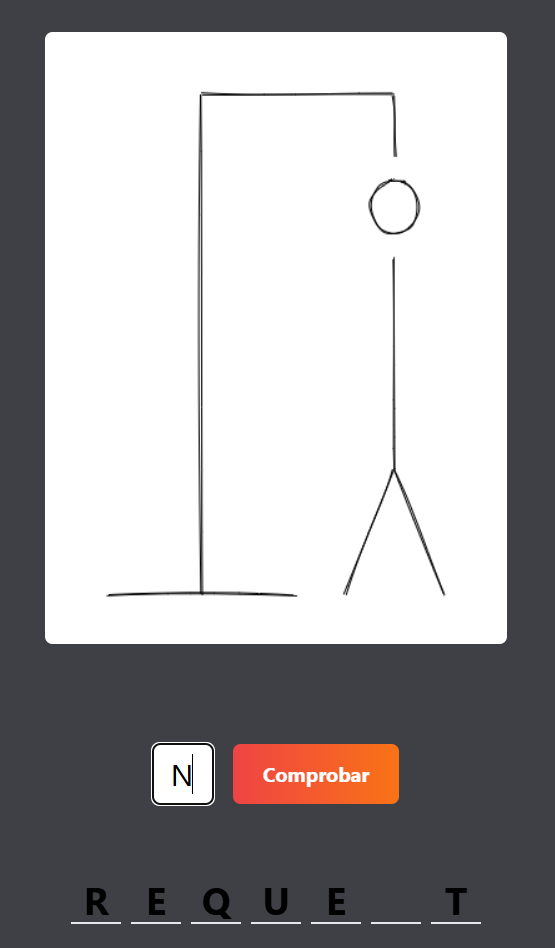
\includegraphics[width=0.3\textwidth,keepaspectratio]{img/prueba.png}
	\caption{Prueba del juego del ahorcado.}
	\centering
	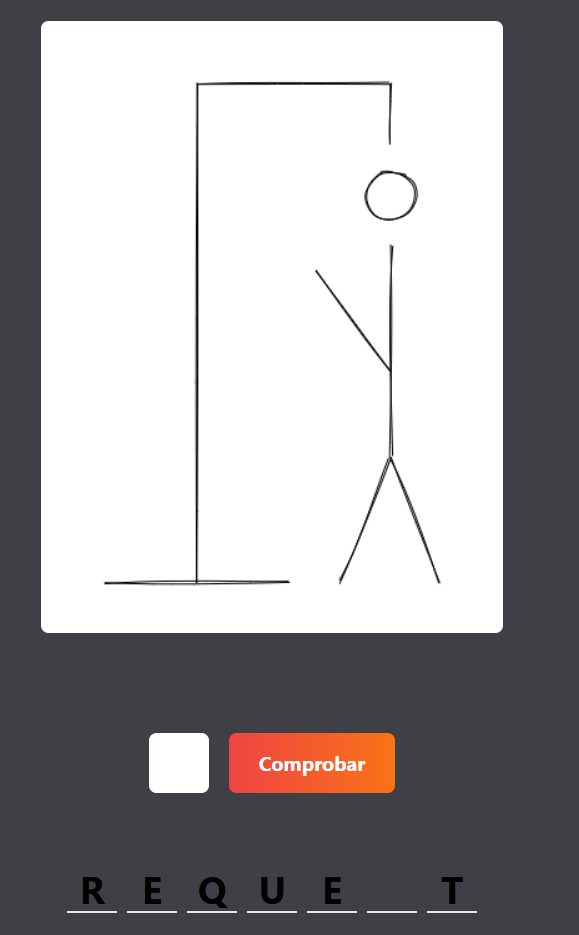
\includegraphics[width=0.3\textwidth,keepaspectratio]{img/prueba2.png}
	\caption{Prueba 2 del juego del ahorcado.}
\end{figure}
\pagebreak

\section{URL del repositorio en GitHub}
\begin{itemize}
	\item \url{https://github.com/Alsnj20/pw2-24a/tree/main/lab09}
\end{itemize}



\section{Estructura de laboratorio \itemPracticeNumber}
\begin{itemize}
	\item El contenido que se entrega en este laboratorio es el siguiente:
\end{itemize}
\begin{lstlisting}{language=bash}
lab09/
	|--Angular/
		|--hangMan/
			|--src/
				|--app/
					|--app.component.ts
					|--app.component.html
					|--app.component.css
					|--canvas/
						|--canvas.component.ts
						|--canvas.component.html
					|--keyboard/
						|--keyboard.component.ts
						|--keyboard.component.html
						|--keyboard.component.css
	|--Latex/
		|--linopinto_pw2_24a_lab09.tex
		|--linopinto_pw2_24a_lab09.pdf
		|--img/
			 |--commits.png
			 |--prueba.png
	|--sciense-quiz/
|--.gitignore
\end{lstlisting}
\section{Rúbrica}
\begin{table}[H]
	\centering
	\caption{Tabla: Rúbrica para contenido del Informe y evidencias}
	\begin{tabular}{|p{2cm}|p{6cm}|c|c|c|c|}
		\hline
		\multicolumn{2}{|c|}{\textbf{Contenido y demostración}} & \textbf{Puntos}                                                                                                                                                                                                                                                                  & \textbf{Checklist} & \textbf{Estudiante} & \textbf{Profesor}   \\ \hline
		1. GitHub                                               & Repositorio se pudo clonar y se evidencia la estructura adecuada para revisar los entregables. (Se descontará puntos por error o observación)                                                                                                                                    & 4                  & ×                   & 4                 & \\ \hline
		2. Commits                                              & Hay porciones de código fuente asociado a los commits planificados con explicaciones detalladas. (El profesor puede preguntar para refrendar calificación)                                                                                                                       & 4                  & ×                   & 4                 & \\ \hline
		3. Ejecución                                            & Se incluyen comandos para ejecuciones y pruebas del código fuente explicadas gradualmente que permitirían replicar el proyecto. (Se descontará puntos por cada omisión)                                                                                                          & 4                  & ×                   & 4                 & \\ \hline
		4. Pregunta                                             & Se responde con completitud a la pregunta formulada en la tarea. (El profesor puede preguntar para refrendar calificación)                                                                                                                                                       & 2                  & ×                   & 2                 & \\ \hline
		7.Ortografía                                            & El documento no muestra errores ortográficos. (Se descontará puntos por error encontrado)                                                                                                                                                                                        & 2                  & ×                   & 1                 & \\ \hline
		8. Madurez                                              & El Informe muestra de manera general una evolución de la madurez del código fuente con explicaciones puntuales pero precisas, agregando diagramas generados a partir del código fuente y refleja un acabado impecable. (El profesor puede preguntar para refrendar calificación) & 4                  & ×                   & 4                 & \\ \hline
		\multicolumn{2}{|c|}{\textbf{Total}}                    & 20                                                                                                                                                                                                                                                                               & Completo           & 19                  &                     \\ \hline
	\end{tabular}
\end{table}

\section{Referencias}
\begin{itemize}
	\item \url{https://github.com/}
	\item \url{https://git-scm.com/}
	\item \url{https://www.w3schools.com/python/}
\end{itemize}

\pagebreak
\end{document}